\documentclass[10pt]{beamer}

\usepackage{bbm}
\usepackage{graphicx}
\graphicspath{{figs/}}
% \epstopdfsetup{outdir=../../figs/}

% \usepackage[backend=bibtex, style=authoryear, defernumbers=true, doi=false, url=false, isbn=false]{biblatex}
%     \renewbibmacro{in:}{}
%     \AtEveryBibitem{\clearfield{month}}
%     \AtEveryBibitem{\clearfield{day}}
%     \addbibresource{StudentLoansChoices.bib}
%     \setbeamertemplate{bibliography item}{}

\setbeamertemplate{section in toc}[sections numbered]

% Define blind footnote (no marker)
\newcommand\blfootnote[1]{%
    \begingroup
    \renewcommand\thefootnote{}\footnote{#1}%
    \addtocounter{footnote}{-1}%
    \endgroup
}

% Increase item sep
\let\OLDitemize\itemize
\renewcommand\itemize{\OLDitemize\addtolength{\itemsep}{.5\baselineskip}}

% Automatically add section slide
\AtBeginSection[]{
  \begin{frame}[noframenumbering, plain, c]
  \vfill
  \centering
  \begin{beamercolorbox}[sep=8pt,center,shadow=true,rounded=true]{title}
    \usebeamerfont{title}\insertsectionhead\par%
  \end{beamercolorbox}
  \vfill
  \end{frame}
}

% Remove navigation buttons and add page numbers
\beamertemplatenavigationsymbolsempty
\setbeamertemplate{footline}[frame number]

% Title matter
\title{Precept 1: \\ Housekeeping \\ Demand \& Supply, pt. 1}
\author{Álvaro Carril\thanks{\url{acarril@princeton.edu}}}
\institute{511c - Microeconomics \\ Princeton University}

\begin{document}

\begin{frame}[noframenumbering, plain, c]
    \maketitle
\end{frame}

\section{Housekeeping}

\begin{frame}{Intros!}
    I'm not a huge fan either, but I believe they are necessary.
    \begin{center}
        
\includegraphics[width=\textwidth]{grief_counseling.png}
    \end{center}
    \textsuperscript{*}That is a joke, \emph{do not give your phone number.}
\end{frame}

\begin{frame}{Evaluations (this precept is going to help you with)}
    \begin{itemize}
        \item \textbf{My job is that you (a) learn and (b) pass.}
        \item The course's evaluations are
        \begin{enumerate}
            \item[20\%] --- Problem sets (\(\sim 10\))
            \item[25\%] --- Policy Analysis presentations (\(\sim 8 \implies 1 \) talk \& discussion per group)
            \item[50\%] --- Midterm \& Exam
            \item[] 
            \item[\(\rightarrow\)] evenly divided between lectures and precept! 
        \end{enumerate}
    \end{itemize}
\end{frame}

\begin{frame}{How this precept is going to help you}
    \begin{itemize}
        \item Focus on math problems, which comprise \(\geq 0.5\) of the problem sets and \(\geq 0.5\) of midterm \& exam.
        \begin{itemize}
            \item[\(\rightarrow\)] Policy Analysis presentations lean more on lectures.
        \end{itemize}
        \item Virtual, live (but recorded) sessions.
        \begin{itemize}
            \item[\(\rightarrow\)] no penalties for not attending live! (but probably better for you)
        \end{itemize}
        \item (Sorry to the people who showed up for a test precept that I scheduled!)
        \item Current time is 10:30 -- 12:00 ET on Friday.
        \begin{itemize}
            \item[\(\rightarrow\)] do we want to change it?
            \item \url{https://www.when2meet.com/?9674172-mnmhS}
        \end{itemize}
    \end{itemize}
    \pause
    \vspace{\baselineskip}
    Any questions about the evaluations?
\end{frame}

\section{Demand \& Supply}

\begin{frame}{Demand}
    \begin{itemize}
        \item A demand curve is an abstraction to represent aggregate willingness to pay.
        \item In other words, it answers ``if the price of something is \(p\), what would be the total amount \(q\) that people would want?''
        \pause
        \item Let's take a look at how this works in practice...
    \end{itemize}
    \begin{center}
        
\includegraphics[width=.5\textwidth]{to-the-juliamobile.jpg}
    \end{center}
\end{frame}

\begin{frame}{Supply}
    \begin{itemize}
        \item The supply curve is an analogous abstraction that now aggregates willingness to \emph{produce} at a given price.
        \item In other words, it answers ``if the price of something is \(p\), what would be the total amount \(q\) that firm(s) would want to produce?''
    \end{itemize}
\end{frame}

\begin{frame}[t]{Problem 1: Yellowteeth Elementary}
    Suppose that the monthly demand and supply for candy in Yellowteeth Elementary are given by
    \begin{align*}
        Q_d(P) &= 300 - 3P + 4I, \\
        Q_s(P) &= 3P - 50,
    \end{align*}
    where \(P\) is price in cents, \(Q\) is total quantity, and \(I\) is some income that students make by organizing different in-school activities (in US\$).
    \begin{enumerate}
        \item[a)] Find the equilibrium price and quantity in this market if \(I = 25\). Draw a plot of the solution.%
        \footnote{Whenever you have to ``plot'' or ``draw'' in these problems, make sure to put named axes, supply and demand curves with correctly signed slopes, and equilibrium price and quantity.}
        What is the consumer's surplus?
    \end{enumerate}
\end{frame}

\begin{frame}[t]{Problem 1: Yellowteeth Elementary}
    \begin{enumerate}
        \item[b)] Suppose now that after a summer of being locked up, kids managed to rise their combined income to \(I = 40\). Without any algebra, can you predict what will happen to the equilibrium (i.e. price and quantity) in this market?
        \item[c)] Compute the new equilibrium price and quantity, and overlay the new demand on the previous figure. Did consumer surplus increase?
    \end{enumerate}
\end{frame}

\begin{frame}{Problem 1: Yellowteeth Elementary}
    \begin{center}
        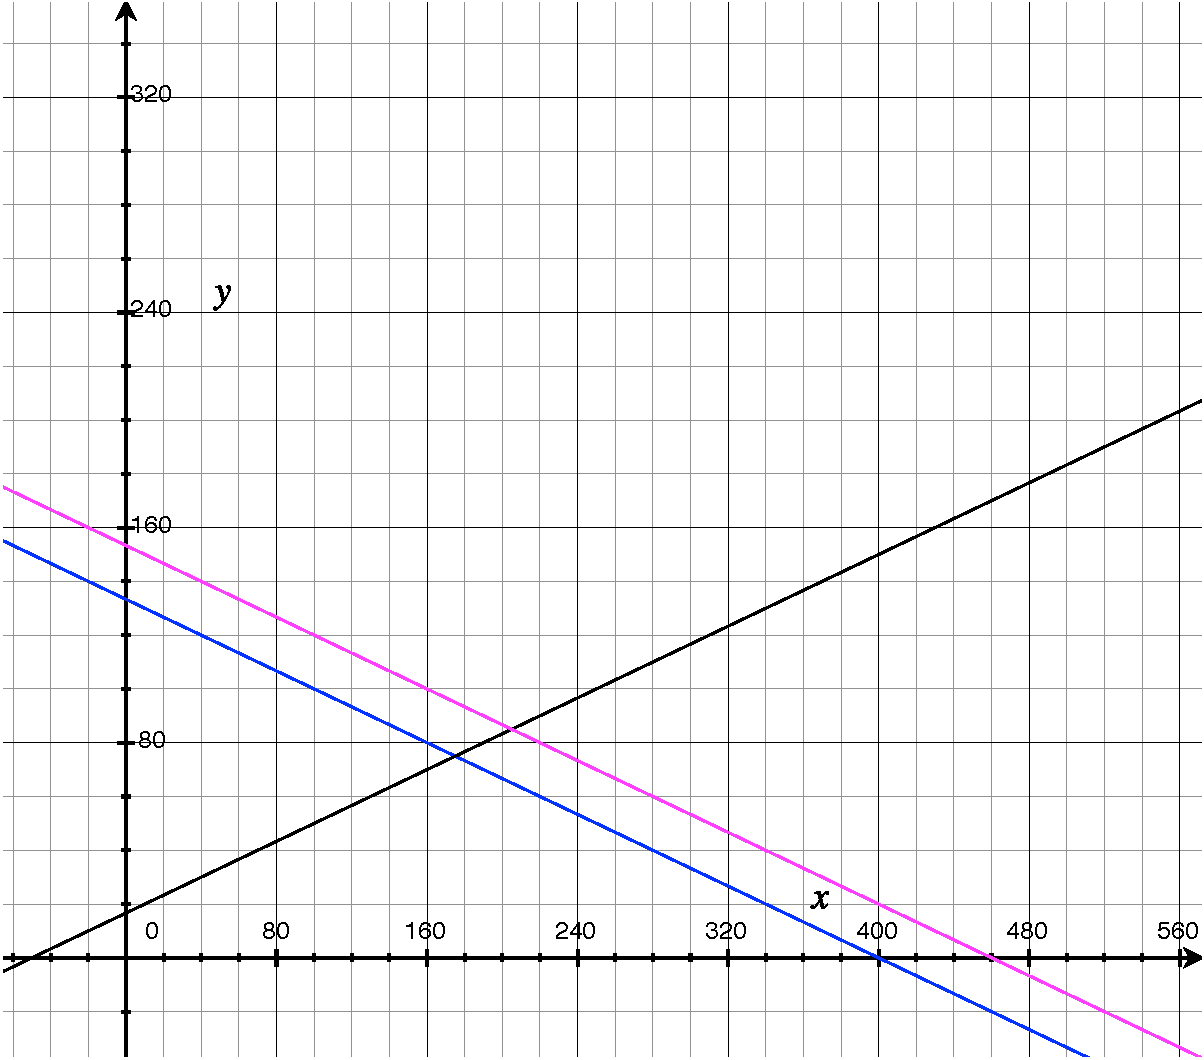
\includegraphics[width=.75\textwidth]{prob1.pdf}
    \end{center}
\end{frame}

\begin{frame}[t]{Problem 1: Yellowteeth Elementary}
    \begin{enumerate}
        \item[d)] Suppose that the principal of Yellowteeth is trying to reduce candy consumption to a total of 160.
        While she can't directly control the supply in the school, she can take some of the in-school income of kids to finance some other activity.
        What is the minimum amount she would have to take away in order to lower total consumption to \(Q^* = 160\)?
        Without doing any algebra, what do you think will happen to consumer surplus?
    \end{enumerate}
\end{frame}

\begin{frame}[t]{Problem 2: NYC apartments}
    The rent control agency of NYC estimates that aggregate demand is
    \begin{equation*}
        Q_d(P) = 160 - 8P,
    \end{equation*}
    where \(Q\) is the quantity, measured in 10,000 apartments, and \(P\) is the average monthly rent, measured in USD100.
    The city's board of realtors estimates the supply is
    \begin{equation*}
        Q_s(P) = 70 + 7P.
    \end{equation*}
    \begin{enumerate}
        \item[a)] What is the equilibrium price in this market? What is the change in city population if the agency sets a maximum average monthly rate of \$300 and all those who cannot find that sweet NYC apartment must leave the city?
    \end{enumerate}
\end{frame}

\begin{frame}{Problem 2: NYC apartments}
    \begin{center}
        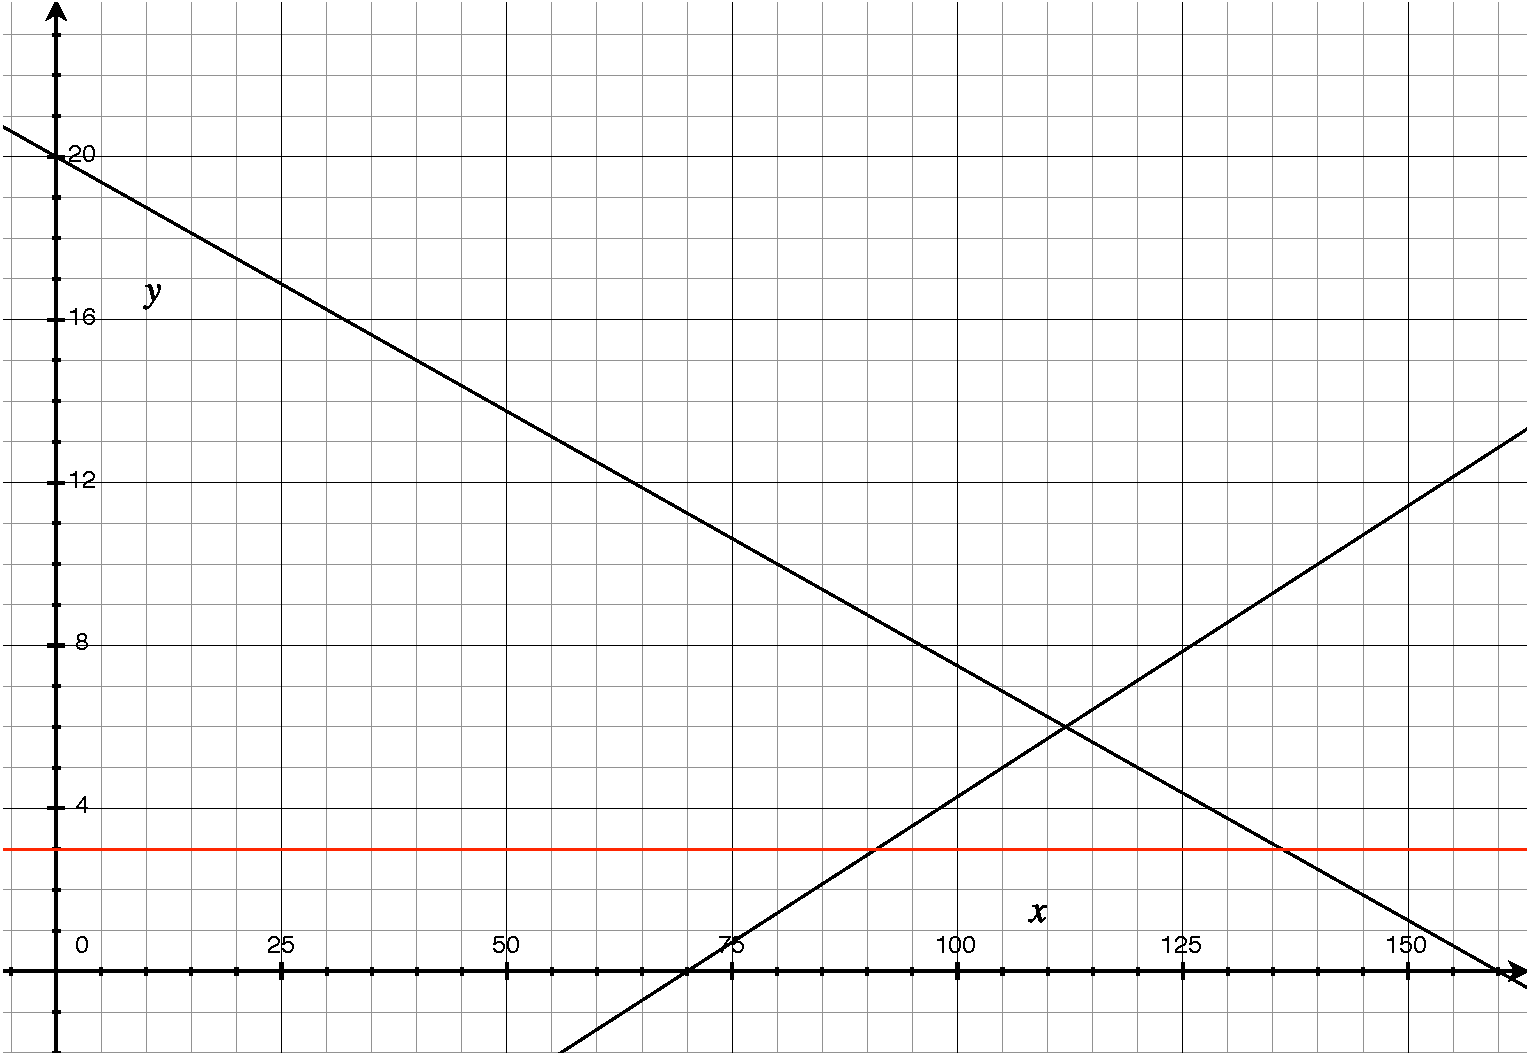
\includegraphics[width=.95\textwidth]{prob2.pdf}
    \end{center}
\end{frame}

\begin{frame}[t]{Problem 2: NYC apartments}
    \begin{enumerate}
        \item[b)] Suppose that the boards puts enough pressure so that the rental price is set to \$900 per month, in order for landlords to have a ``fair'' rate of return.
        If 50\% of any long-run increases in apartment offerings comes from new construction, how many new apartments are constructed? 
    \end{enumerate}
\end{frame}

\begin{frame}{Problem 3: Netflix\footnote{Netflix evidently has significant market power in the video streaming market, but I'm ignoring that until we see it in class.}}
    Netflix is one of the few companies actually thriving during the coronavirus.
    It is now worth \$194b, increasing its value by 35\% since March 2020.

    The government estimates that the demand faced by Netflix is
    \begin{equation}
        P(Q_d) = 12 - 0.5Q_d + \mathbbm{1}_{\text{Office}} (4 + 1.5Q_d),
    \end{equation}
    where \(\mathbbm{1}_{\text{Office}}\) is an indicator function that is equal to 1 if Netflix offers The Office, and 0 if it doesn't.
    Netflix's(?) supply curve is
    \begin{equation}
        P(Q_s) = 6 + 0.5Q_s.
    \end{equation}
\end{frame}

\begin{frame}[t]{Problem 3: Netflix}
    \begin{enumerate}
        \item[a)] Suppose that we're still in year 2020 (*sigh*), and Netflix can still show The Office. What is the equilibrium price and quantity in this market?
    \end{enumerate}
\end{frame}

\begin{frame}[t]{Problem 3: Netflix}
    \begin{enumerate}
        \item[b)] In an effort to finance cash stimulus for poor families, the government is considering the approval of a ``Netflix tax'', which would tax the supply with \$2.5.
        What would be the total revenue collected from this tax? What would each side of the market be paying? 
    \end{enumerate}
\end{frame}

\begin{frame}{Problem 3: Netflix}
    \begin{center}
        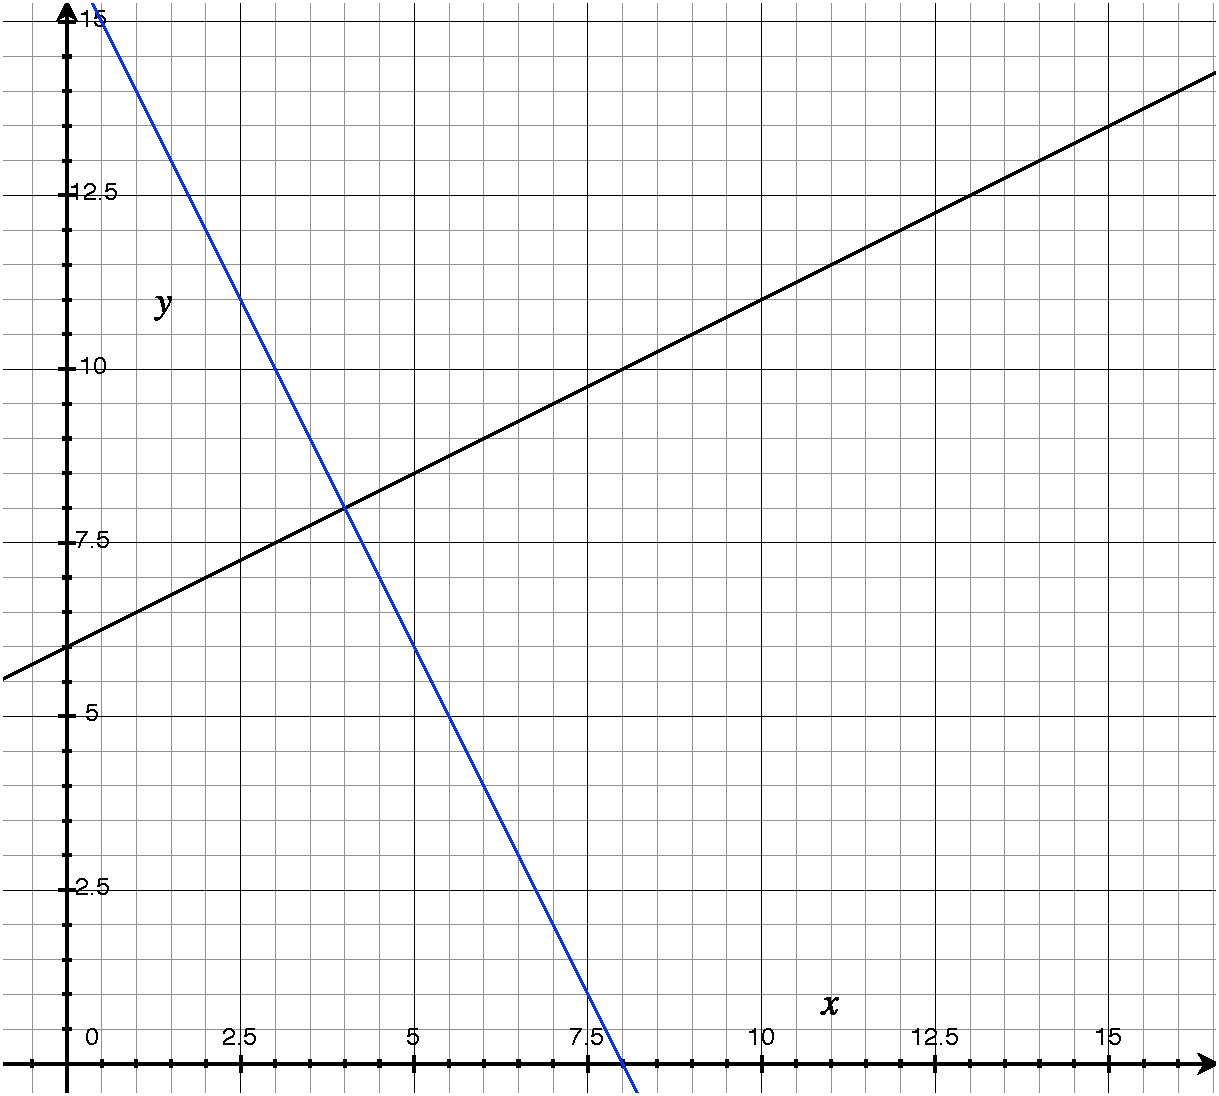
\includegraphics[width=.75\textwidth]{prob3_1.pdf}
    \end{center}
\end{frame}

\begin{frame}[t]{Problem 3: Netflix}
    \begin{enumerate}
        \item[c)] Suppose now that year 2020 is over and Netlfix no longer can play The Office.
        Comment how would your answer in b) change, and what is the reason behind those changes, if any.
    \end{enumerate}
\end{frame}

\begin{frame}{Problem 3: Netflix}
    \begin{center}
        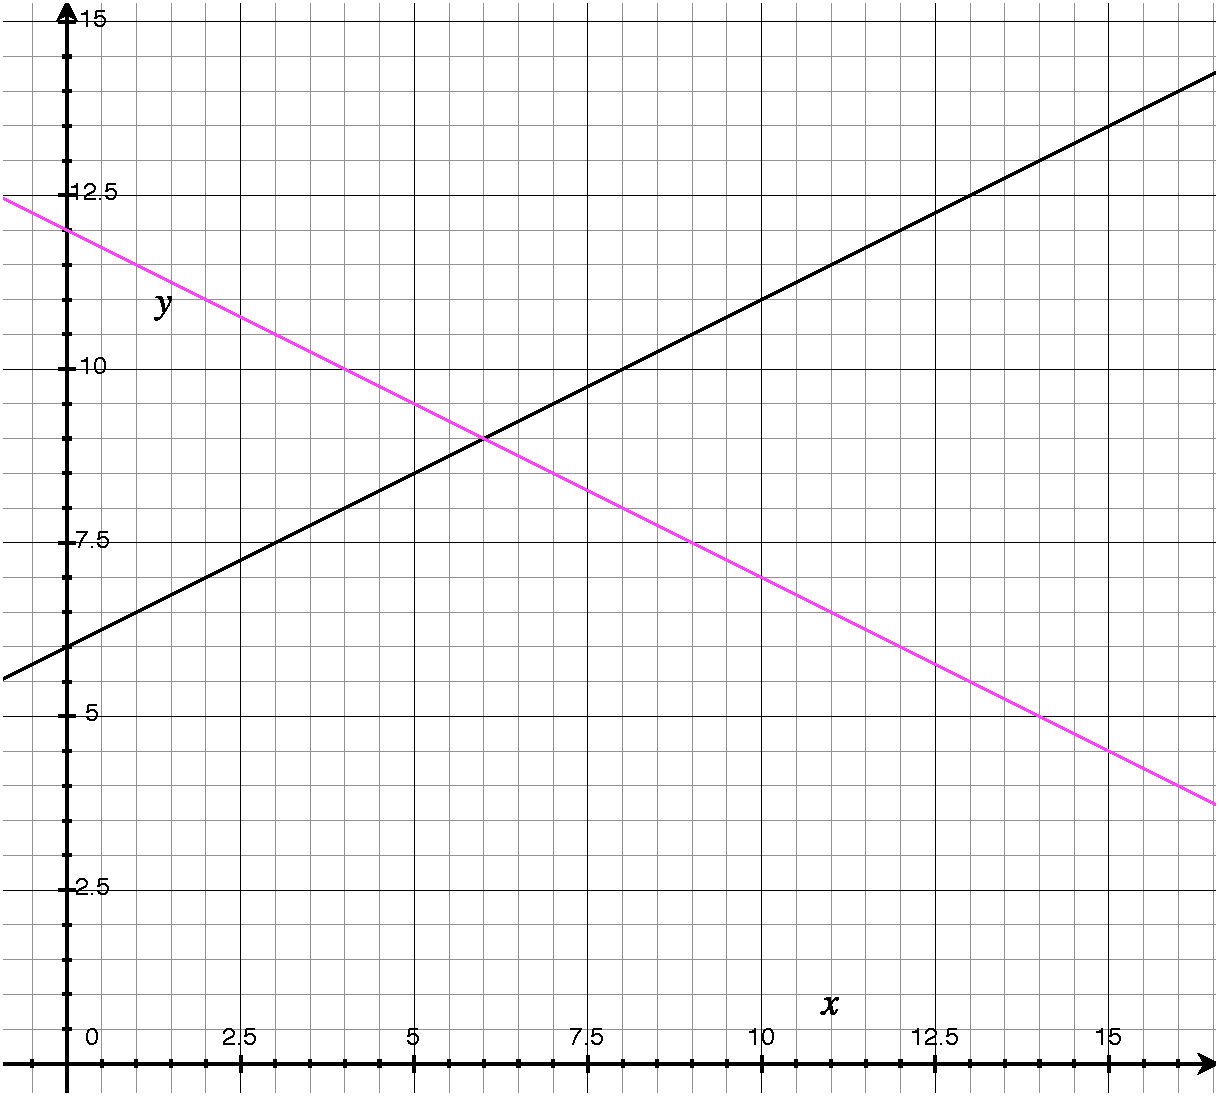
\includegraphics[width=.75\textwidth]{prob3_2.pdf}
    \end{center}
\end{frame}

% \begin{frame}[t]{Problem 1}
%     Let \(u(\cdot)\) denote Alvaro's utility function.
%     We know Alvaro derives utility solely from pizza slices and beers.
%     His utility function is
%     \begin{equation}
%         u(x, y) = \sqrt{x \cdot y},
%         \label{eq:utility_Alvaro}
%     \end{equation}
%     where \(x\) is the number of pizza slices and \(y\) is the number of beers.

%     \begin{enumerate}
%         \item[a)] Sketch Alvaro's indifference curves for \(u = \{2, 8, 16\}\). Do you notice a pattern as \((x, y)\) increase? Is there a (reasonable) economic interpretation for it?
%     \end{enumerate}
% \end{frame}

% \begin{frame}[c]
%     \begin{figure}
%         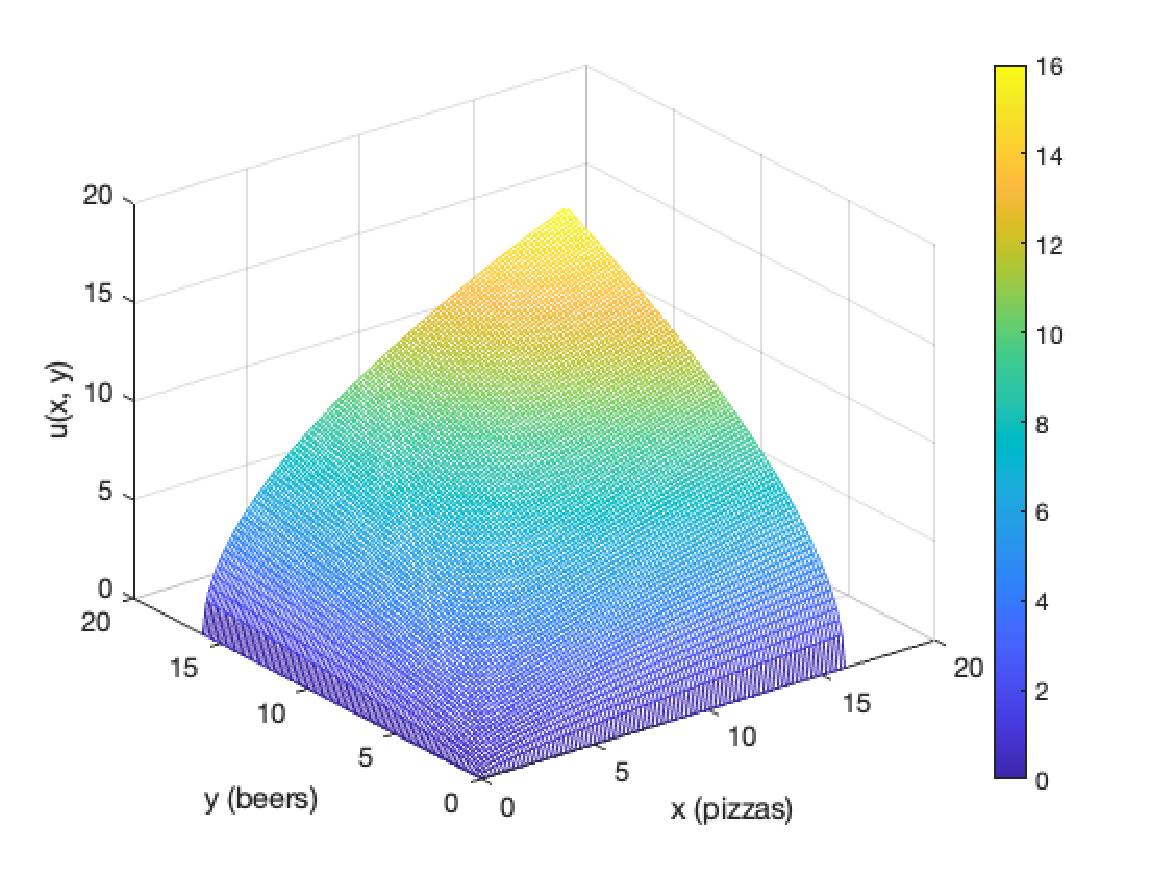
\includegraphics[width=\textwidth]{plot_utility_3dmesh.pdf}
%         \caption{Plot of utility function in \eqref{eq:utility_Alvaro} on a \(16 \times 16\) mesh grid}
%     \end{figure}
% \end{frame}

% \begin{frame}[c]
%     \begin{figure}
%         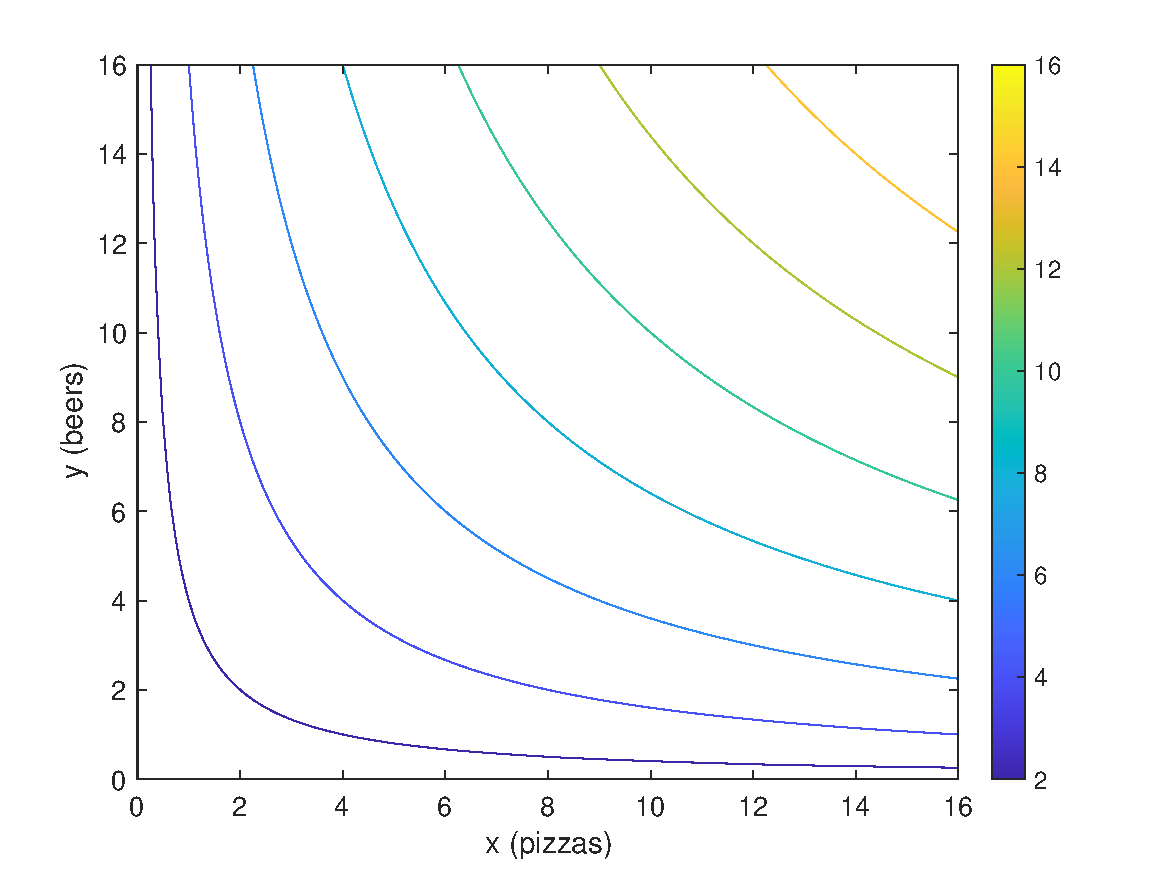
\includegraphics[width=\textwidth]{contour_utility_Alvaro.pdf}
%         \caption{Plot of utility function in \eqref{eq:utility_Alvaro} on a \(16 \times 16\) mesh grid}
%     \end{figure}
% \end{frame}

% \begin{frame}[c]{Problem 1}
%     The current utility function:
%     \begin{figure}
%         \centering
%         
\includegraphics[width=.6\textwidth]{balanced.png}
%     \end{figure}
% \end{frame}

% \begin{frame}[t]{Problem 1}
%     Suppose Alvaro's utility function actually is
%     \begin{equation}
%         u(x, y) = x^{0.3} \cdot y^{0.7},
%         \label{eq:utility_Alvaro}
%     \end{equation}

%     \begin{enumerate}
%         \item[b)] Again, sketch Alvaro's indifference curves for \(u = \{2, 8, 16\}\), contrasting it with the previous case.
%     \end{enumerate}
% \end{frame}

\begin{frame}{Wrapping up}
    \begin{itemize}
        \item Demand and supply are useful abstractions, but not a perfect representation of reality.
        \item Models that are simplified versions of reality are useful---learning to think within the model's framework is key.
        \item Liked the code? Want to play a bit more with it? I'll upload everything I do in this precept to \url{https://github.com/acarril/511c_notebooks}.
        \item Did I do good, meh, bad? Tell me anonymously! Or not. But always remember I have feelings :)\vspace{\baselineskip}
        \url{https://forms.gle/8xtjP1XQzUNwovTy6}
    \end{itemize}
    \vspace{\baselineskip}Thank you!
\end{frame}

\end{document}
